\chapter{Example Systems}\label{ch:systems}

Reservoir computers are most useful as tools for answering questions
about dynamic systems, such as state inference and
forecasting. Throughout this thesis, I use many small chaotic systems
for example RC tasks. For reference, they are included here.

\section{Lorenz '63}\label{sec:lorenz}

\begin{figure}
  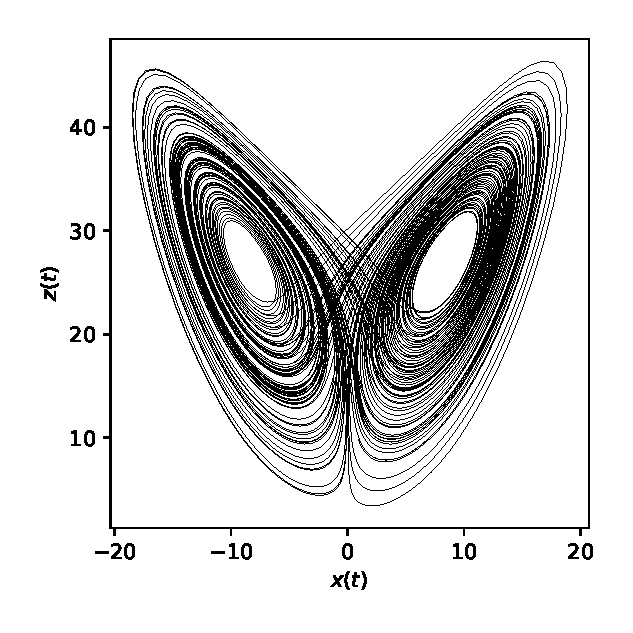
\includegraphics[width=0.6\textwidth]{figures/lorenz}
  \caption{The true Lorenz attractor in the $x$/$z$ plane, produced by integrating \cref{eq:lorenz}.}%
  \label{fig:lorenz}
\end{figure}

The Lorenz '63 chaotic system is described by
\begin{equation}
  \begin{aligned}
    \dot{x} &= 10 \left(y - x\right), \\
    \dot{y} &= x \left(28 - z\right) - y, \\
    \dot{z} &= x\,y - \frac{8}{3} z,
  \end{aligned}
  \label{eq:lorenz}
\end{equation}
with standard parameters.\cite{lorenz1963} The attractor of this
system can be visualized easily in two dimensions by projecting the
three-dimensional trajectory of the system onto a plane. I show the
attractor in the $x$/$z$ plane in \cref{fig:lorenz}.

\section{R{\"{o}}ssler}\label{sec:rossler}

\begin{figure}
  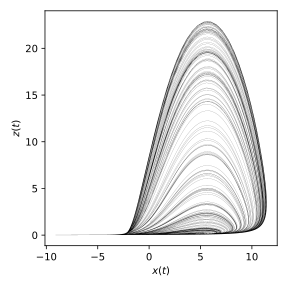
\includegraphics[width=0.6\textwidth]{figures/rossler}
  \caption{The true R{\"{o}}ssler attractor in the $x$/$z$ plane, produced by integrating \cref{eq:rossler}.}%
  \label{fig:rossler}
\end{figure}

The R{\"{o}}ssler system is described by
\begin{equation}
  \begin{aligned}
    \dot{x} &= - y - z, \\
    \dot{y} &= x + a y, \\
    \dot{z} &= b + z (x - c),
  \end{aligned}
  \label{eq:rossler}
\end{equation}
with standard parameters $a = 0.2$, $b = 0.2$, $c =
5.7$.\cite{rossler1976} The attractor of this system is visualized in
\cref{fig:rossler}.

The $z$ component of this system mostly stays near zero, with rare
positive spikes. This makes prediction with an RC difficult. To make
this component of the system more suitable for RC prediction, I use
$\log z$ instead for both RC input and prediction output.

\section{Double-Scroll}\label{sec:dscroll}

\begin{figure}
  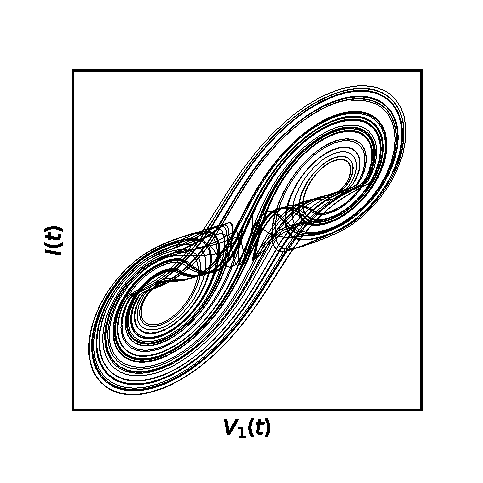
\includegraphics[width=0.6\textwidth]{figures/dscroll}
  \caption{The true double-scroll circuit attractor in the $V_1$/$I$ plane, produced by integrating \cref{eq:dscroll}.}%
  \label{fig:dscroll}
\end{figure}

The double-scroll chaotic circuit is described by the dimensionless equations
\begin{equation}
 \begin{aligned}
   \dot{V_1} &= \frac{V_1}{R_1} - \frac{V_1 - V_2}{R_2} - 2 I_r \sinh\left(\alpha(V_1 - V_2)\right), \\
   \dot{V_2} &= \frac{V_1 - V_2}{R_2} + 2 I_r \sinh\left(\alpha(V_1 - V_2)\right) - I, \\
   \dot{I} &= V_2 - R_4 I,
 \end{aligned}
 \label{eq:dscroll}
\end{equation}
with parameters $R_1 = 1.2$, $R_2 = 3.44$, $R_4 = 0.193$, $I_r = 2.25
\times 10^{-5}$, and $\alpha = 11.6$.\cite{gauthier1996} The attractor
of this system is visualized in \cref{fig:dscroll}.

\section{Mackey-Glass}\label{sec:mackey-glass}

\begin{figure}
  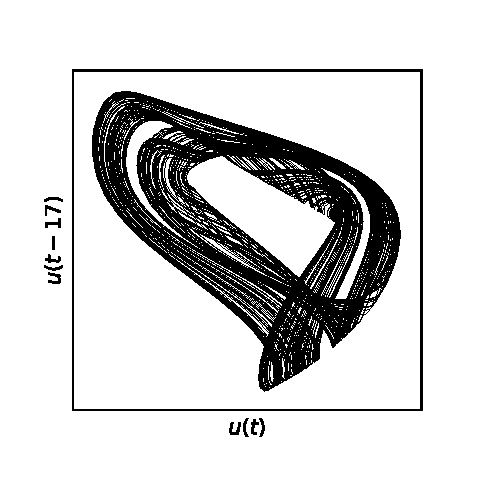
\includegraphics[width=0.6\textwidth]{figures/mackey-glass}
  \caption{The true Mackey-Glass attractor represented as a time delay embedding using $\tau$ as the delay, produced by integrating \cref{eq:mackey-glass}.}%
  \label{fig:mackey-glass}
\end{figure}

The Mackey-Glass system is described by the time-delay differential equation
\begin{equation}
  \dot{u}(t) = \beta \frac{u(t - \tau)}{1 + u(t - \tau)^n} - \gamma u(t),
  \label{eq:mackey-glass}
\end{equation}
with standard parameters $\beta = 0.2$, $\gamma = 0.1$, $\tau = 17$,
$n = 10$.\cite{mackey1977} The attractor of this system is most
commonly visualized as a time-delay embedding of the trajectory, using
$\tau$ as the delay parameter, as depicted in \cref{fig:mackey-glass}.
